% Options for packages loaded elsewhere
\PassOptionsToPackage{unicode}{hyperref}
\PassOptionsToPackage{hyphens}{url}
%
\documentclass[
]{article}
\usepackage{lmodern}
\usepackage{amssymb,amsmath}
\usepackage{ifxetex,ifluatex}
\ifnum 0\ifxetex 1\fi\ifluatex 1\fi=0 % if pdftex
  \usepackage[T1]{fontenc}
  \usepackage[utf8]{inputenc}
  \usepackage{textcomp} % provide euro and other symbols
\else % if luatex or xetex
  \usepackage{unicode-math}
  \defaultfontfeatures{Scale=MatchLowercase}
  \defaultfontfeatures[\rmfamily]{Ligatures=TeX,Scale=1}
\fi
% Use upquote if available, for straight quotes in verbatim environments
\IfFileExists{upquote.sty}{\usepackage{upquote}}{}
\IfFileExists{microtype.sty}{% use microtype if available
  \usepackage[]{microtype}
  \UseMicrotypeSet[protrusion]{basicmath} % disable protrusion for tt fonts
}{}
\makeatletter
\@ifundefined{KOMAClassName}{% if non-KOMA class
  \IfFileExists{parskip.sty}{%
    \usepackage{parskip}
  }{% else
    \setlength{\parindent}{0pt}
    \setlength{\parskip}{6pt plus 2pt minus 1pt}}
}{% if KOMA class
  \KOMAoptions{parskip=half}}
\makeatother
\usepackage{xcolor}
\IfFileExists{xurl.sty}{\usepackage{xurl}}{} % add URL line breaks if available
\IfFileExists{bookmark.sty}{\usepackage{bookmark}}{\usepackage{hyperref}}
\hypersetup{
  pdftitle={Oblig 1},
  hidelinks,
  pdfcreator={LaTeX via pandoc}}
\urlstyle{same} % disable monospaced font for URLs
\usepackage[margin=1in]{geometry}
\usepackage{color}
\usepackage{fancyvrb}
\newcommand{\VerbBar}{|}
\newcommand{\VERB}{\Verb[commandchars=\\\{\}]}
\DefineVerbatimEnvironment{Highlighting}{Verbatim}{commandchars=\\\{\}}
% Add ',fontsize=\small' for more characters per line
\usepackage{framed}
\definecolor{shadecolor}{RGB}{248,248,248}
\newenvironment{Shaded}{\begin{snugshade}}{\end{snugshade}}
\newcommand{\AlertTok}[1]{\textcolor[rgb]{0.94,0.16,0.16}{#1}}
\newcommand{\AnnotationTok}[1]{\textcolor[rgb]{0.56,0.35,0.01}{\textbf{\textit{#1}}}}
\newcommand{\AttributeTok}[1]{\textcolor[rgb]{0.77,0.63,0.00}{#1}}
\newcommand{\BaseNTok}[1]{\textcolor[rgb]{0.00,0.00,0.81}{#1}}
\newcommand{\BuiltInTok}[1]{#1}
\newcommand{\CharTok}[1]{\textcolor[rgb]{0.31,0.60,0.02}{#1}}
\newcommand{\CommentTok}[1]{\textcolor[rgb]{0.56,0.35,0.01}{\textit{#1}}}
\newcommand{\CommentVarTok}[1]{\textcolor[rgb]{0.56,0.35,0.01}{\textbf{\textit{#1}}}}
\newcommand{\ConstantTok}[1]{\textcolor[rgb]{0.00,0.00,0.00}{#1}}
\newcommand{\ControlFlowTok}[1]{\textcolor[rgb]{0.13,0.29,0.53}{\textbf{#1}}}
\newcommand{\DataTypeTok}[1]{\textcolor[rgb]{0.13,0.29,0.53}{#1}}
\newcommand{\DecValTok}[1]{\textcolor[rgb]{0.00,0.00,0.81}{#1}}
\newcommand{\DocumentationTok}[1]{\textcolor[rgb]{0.56,0.35,0.01}{\textbf{\textit{#1}}}}
\newcommand{\ErrorTok}[1]{\textcolor[rgb]{0.64,0.00,0.00}{\textbf{#1}}}
\newcommand{\ExtensionTok}[1]{#1}
\newcommand{\FloatTok}[1]{\textcolor[rgb]{0.00,0.00,0.81}{#1}}
\newcommand{\FunctionTok}[1]{\textcolor[rgb]{0.00,0.00,0.00}{#1}}
\newcommand{\ImportTok}[1]{#1}
\newcommand{\InformationTok}[1]{\textcolor[rgb]{0.56,0.35,0.01}{\textbf{\textit{#1}}}}
\newcommand{\KeywordTok}[1]{\textcolor[rgb]{0.13,0.29,0.53}{\textbf{#1}}}
\newcommand{\NormalTok}[1]{#1}
\newcommand{\OperatorTok}[1]{\textcolor[rgb]{0.81,0.36,0.00}{\textbf{#1}}}
\newcommand{\OtherTok}[1]{\textcolor[rgb]{0.56,0.35,0.01}{#1}}
\newcommand{\PreprocessorTok}[1]{\textcolor[rgb]{0.56,0.35,0.01}{\textit{#1}}}
\newcommand{\RegionMarkerTok}[1]{#1}
\newcommand{\SpecialCharTok}[1]{\textcolor[rgb]{0.00,0.00,0.00}{#1}}
\newcommand{\SpecialStringTok}[1]{\textcolor[rgb]{0.31,0.60,0.02}{#1}}
\newcommand{\StringTok}[1]{\textcolor[rgb]{0.31,0.60,0.02}{#1}}
\newcommand{\VariableTok}[1]{\textcolor[rgb]{0.00,0.00,0.00}{#1}}
\newcommand{\VerbatimStringTok}[1]{\textcolor[rgb]{0.31,0.60,0.02}{#1}}
\newcommand{\WarningTok}[1]{\textcolor[rgb]{0.56,0.35,0.01}{\textbf{\textit{#1}}}}
\usepackage{graphicx,grffile}
\makeatletter
\def\maxwidth{\ifdim\Gin@nat@width>\linewidth\linewidth\else\Gin@nat@width\fi}
\def\maxheight{\ifdim\Gin@nat@height>\textheight\textheight\else\Gin@nat@height\fi}
\makeatother
% Scale images if necessary, so that they will not overflow the page
% margins by default, and it is still possible to overwrite the defaults
% using explicit options in \includegraphics[width, height, ...]{}
\setkeys{Gin}{width=\maxwidth,height=\maxheight,keepaspectratio}
% Set default figure placement to htbp
\makeatletter
\def\fps@figure{htbp}
\makeatother
\setlength{\emergencystretch}{3em} % prevent overfull lines
\providecommand{\tightlist}{%
  \setlength{\itemsep}{0pt}\setlength{\parskip}{0pt}}
\setcounter{secnumdepth}{-\maxdimen} % remove section numbering

\title{Oblig 1}
\author{}
\date{\vspace{-2.5em}}

\begin{document}
\maketitle

\hypertarget{problem-1}{%
\subsection{Problem 1}\label{problem-1}}

Aim: Find how well bmi, easily computed as the ratio between weight and
squared hight (so mesured in kg/m\^{}2), can be used to predict pbfm,
whose measurment involves instead a bioelectrical impedance analysis.

\hypertarget{a}{%
\subsubsection{a}\label{a}}

Plotting \textbf{bnp} against \textbf{pbfm}, and fitting a simple linear
model with a summary.

\begin{Shaded}
\begin{Highlighting}[]
\KeywordTok{plot}\NormalTok{(bmi, pbfm)}
\NormalTok{fit.simpleLinear <-}\StringTok{ }\KeywordTok{lm}\NormalTok{(pbfm }\OperatorTok{~}\StringTok{ }\NormalTok{bmi)}
\KeywordTok{print}\NormalTok{(}\KeywordTok{summary}\NormalTok{(fit.simpleLinear))}
\end{Highlighting}
\end{Shaded}

\begin{verbatim}
## 
## Call:
## lm(formula = pbfm ~ bmi)
## 
## Residuals:
##      Min       1Q   Median       3Q      Max 
## -16.5116  -2.0714   0.4083   2.4994   9.1758 
## 
## Coefficients:
##             Estimate Std. Error t value Pr(>|t|)    
## (Intercept) 14.82772    0.82671   17.94   <2e-16 ***
## bmi          0.88481    0.02589   34.17   <2e-16 ***
## ---
## Signif. codes:  0 '***' 0.001 '**' 0.01 '*' 0.05 '.' 0.1 ' ' 1
## 
## Residual standard error: 3.702 on 325 degrees of freedom
## Multiple R-squared:  0.7823, Adjusted R-squared:  0.7816 
## F-statistic:  1168 on 1 and 325 DF,  p-value: < 2.2e-16
\end{verbatim}

\begin{Shaded}
\begin{Highlighting}[]
\NormalTok{x =}\StringTok{ }\NormalTok{(}\KeywordTok{seq}\NormalTok{(}\KeywordTok{min}\NormalTok{(bmi), }\KeywordTok{max}\NormalTok{(bmi), }\DataTypeTok{length =} \DecValTok{200}\NormalTok{))}
\NormalTok{beta =}\StringTok{ }\KeywordTok{coef}\NormalTok{(fit.simpleLinear)}
\KeywordTok{lines}\NormalTok{(x, beta[}\DecValTok{1}\NormalTok{] }\OperatorTok{+}\StringTok{ }\NormalTok{beta[}\DecValTok{2}\NormalTok{]}\OperatorTok{*}\StringTok{ }\NormalTok{x, }\DataTypeTok{col =} \DecValTok{2}\NormalTok{, }\DataTypeTok{lty =} \DecValTok{1}\NormalTok{, }\DataTypeTok{lwd =} \DecValTok{2}\NormalTok{)}
\end{Highlighting}
\end{Shaded}

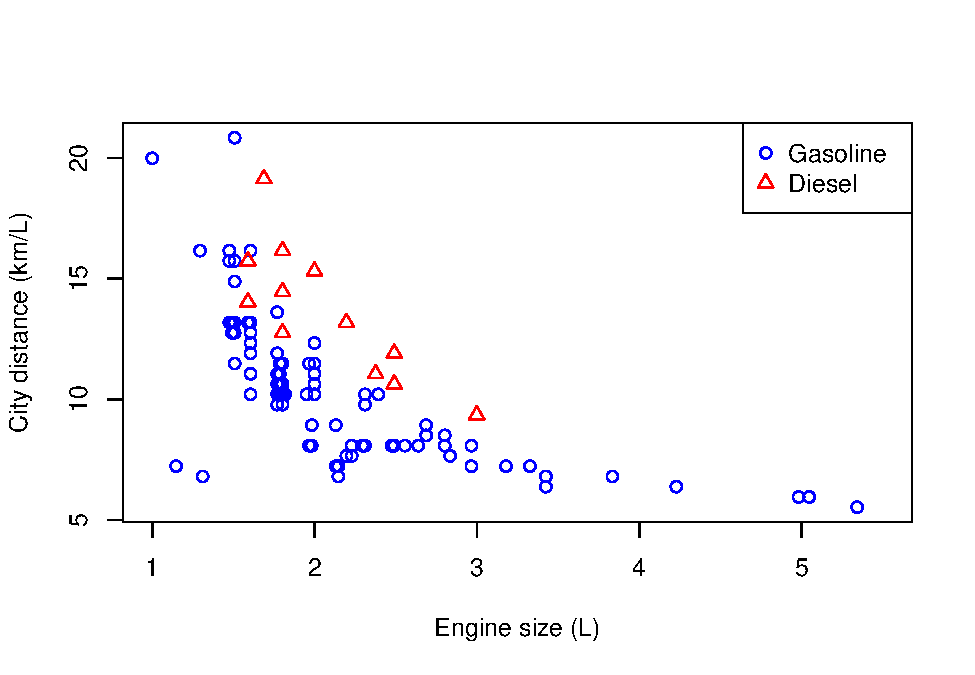
\includegraphics{oblig1_files/figure-latex/unnamed-chunk-2-1.pdf} A
linear model seems ok in the center of the bmi. But it is quite off in
the lower 1/4 and in the upper 1/4.We can see that the intercept and bmi
is strongly significant, indicating a strong correlation between bmi and
pdfm. The R-squared is siginificant, but not super high, so the model
can probably be improved. To see this clearly we plott indicitative
plotts on the fitness.

\begin{Shaded}
\begin{Highlighting}[]
\KeywordTok{plot}\NormalTok{(fit.simpleLinear)}
\end{Highlighting}
\end{Shaded}

\includegraphics{oblig1_files/figure-latex/unnamed-chunk-3-1.pdf}
\includegraphics{oblig1_files/figure-latex/unnamed-chunk-3-2.pdf}
\includegraphics{oblig1_files/figure-latex/unnamed-chunk-3-3.pdf}
\includegraphics{oblig1_files/figure-latex/unnamed-chunk-3-4.pdf}

\hypertarget{residuals-vs-fitted}{%
\paragraph{Residuals vs Fitted}\label{residuals-vs-fitted}}

Shows the Anscombe plot, wich would idealy present a eaven scattering
with no patterns in the points. In the plott we see a clear pattern, and
is indicating possiple violation of homoscedasicity. Meaning that
\epsiplon must be independent of the index.

\hypertarget{normal-q-q}{%
\paragraph{Normal Q-Q}\label{normal-q-q}}

This plot shows quantile-quantile plot. This plot shows the values of
the resiuals in increasing order. To see if the residuals folows a
normal distribution. For the assumption of normality to be valid we
would expect the values to folow the line in the plot. In the plot a
heavy tail and head can be observed. So the assumtion of normality is
not strong.

\hypertarget{scale-location}{%
\paragraph{Scale-Location}\label{scale-location}}

\hypertarget{residual-vs-leverage}{%
\paragraph{Residual vs Leverage}\label{residual-vs-leverage}}

\hypertarget{b}{%
\subsection{b}\label{b}}

We can see that we dont have any negative number, in such cases it is
often benefital to use a logarithmic transformation.

\begin{Shaded}
\begin{Highlighting}[]
\NormalTok{fit.log <-}\StringTok{ }\KeywordTok{lm}\NormalTok{(pbfm }\OperatorTok{~}\StringTok{ }\KeywordTok{log}\NormalTok{(bmi))}
\KeywordTok{print}\NormalTok{(}\KeywordTok{summary}\NormalTok{(fit.log))}
\end{Highlighting}
\end{Shaded}

\begin{verbatim}
## 
## Call:
## lm(formula = pbfm ~ log(bmi))
## 
## Residuals:
##      Min       1Q   Median       3Q      Max 
## -10.2548  -2.0453   0.1026   2.1238   8.6029 
## 
## Coefficients:
##             Estimate Std. Error t value Pr(>|t|)    
## (Intercept) -55.7327     2.3337  -23.88   <2e-16 ***
## log(bmi)     28.8031     0.6845   42.08   <2e-16 ***
## ---
## Signif. codes:  0 '***' 0.001 '**' 0.01 '*' 0.05 '.' 0.1 ' ' 1
## 
## Residual standard error: 3.125 on 325 degrees of freedom
## Multiple R-squared:  0.8449, Adjusted R-squared:  0.8444 
## F-statistic:  1771 on 1 and 325 DF,  p-value: < 2.2e-16
\end{verbatim}

\begin{Shaded}
\begin{Highlighting}[]
\NormalTok{beta =}\StringTok{ }\KeywordTok{coef}\NormalTok{(fit.log)}

\NormalTok{x =}\StringTok{ }\KeywordTok{log}\NormalTok{(}\KeywordTok{seq}\NormalTok{(}\KeywordTok{min}\NormalTok{(bmi), }\KeywordTok{max}\NormalTok{(bmi), }\DataTypeTok{length =} \DecValTok{200}\NormalTok{))}
\KeywordTok{plot}\NormalTok{(bmi, pbfm)}
\KeywordTok{lines}\NormalTok{(}\KeywordTok{exp}\NormalTok{(x),( beta[}\DecValTok{1}\NormalTok{] }\OperatorTok{+}\StringTok{ }\NormalTok{beta[}\DecValTok{2}\NormalTok{]}\OperatorTok{*}\StringTok{ }\NormalTok{x), }\DataTypeTok{col =} \DecValTok{2}\NormalTok{) }
\end{Highlighting}
\end{Shaded}

\includegraphics{oblig1_files/figure-latex/unnamed-chunk-4-1.pdf}

And to see how good the model is we plot some helping plots

\begin{Shaded}
\begin{Highlighting}[]
\KeywordTok{plot}\NormalTok{(fit.log)}
\end{Highlighting}
\end{Shaded}

\includegraphics{oblig1_files/figure-latex/unnamed-chunk-5-1.pdf}
\includegraphics{oblig1_files/figure-latex/unnamed-chunk-5-2.pdf}
\includegraphics{oblig1_files/figure-latex/unnamed-chunk-5-3.pdf}
\includegraphics{oblig1_files/figure-latex/unnamed-chunk-5-4.pdf}

It was also suggested to use a quadratic model.

\begin{Shaded}
\begin{Highlighting}[]
\NormalTok{fit.quad<-}\StringTok{ }\KeywordTok{lm}\NormalTok{(pbfm }\OperatorTok{~}\StringTok{ }\NormalTok{bmi }\OperatorTok{+}\StringTok{ }\KeywordTok{I}\NormalTok{(bmi}\OperatorTok{^}\DecValTok{2}\NormalTok{))}
\KeywordTok{print}\NormalTok{(}\KeywordTok{summary}\NormalTok{(fit.quad))}
\end{Highlighting}
\end{Shaded}

\begin{verbatim}
## 
## Call:
## lm(formula = pbfm ~ bmi + I(bmi^2))
## 
## Residuals:
##     Min      1Q  Median      3Q     Max 
## -9.3403 -1.9246  0.1433  1.8665  8.3780 
## 
## Coefficients:
##              Estimate Std. Error t value Pr(>|t|)    
## (Intercept) -11.17790    2.16977  -5.152 4.49e-07 ***
## bmi           2.53223    0.13229  19.142  < 2e-16 ***
## I(bmi^2)     -0.02448    0.00194 -12.617  < 2e-16 ***
## ---
## Signif. codes:  0 '***' 0.001 '**' 0.01 '*' 0.05 '.' 0.1 ' ' 1
## 
## Residual standard error: 3.036 on 324 degrees of freedom
## Multiple R-squared:  0.854,  Adjusted R-squared:  0.8531 
## F-statistic: 947.8 on 2 and 324 DF,  p-value: < 2.2e-16
\end{verbatim}

\begin{Shaded}
\begin{Highlighting}[]
\NormalTok{beta =}\StringTok{ }\KeywordTok{coef}\NormalTok{(fit.quad)}

\NormalTok{x =}\StringTok{ }\NormalTok{(}\KeywordTok{seq}\NormalTok{(}\KeywordTok{min}\NormalTok{(bmi), }\KeywordTok{max}\NormalTok{(bmi), }\DataTypeTok{length =} \DecValTok{200}\NormalTok{))}
\KeywordTok{plot}\NormalTok{(bmi, pbfm)}
\CommentTok{#points(bmi, pbfm)}
\KeywordTok{lines}\NormalTok{(x, beta[}\DecValTok{1}\NormalTok{] }\OperatorTok{+}\StringTok{ }\NormalTok{beta[}\DecValTok{2}\NormalTok{]}\OperatorTok{*}\NormalTok{x }\OperatorTok{+}\StringTok{ }\NormalTok{beta[}\DecValTok{3}\NormalTok{]}\OperatorTok{*}\NormalTok{x}\OperatorTok{^}\DecValTok{2}\NormalTok{, }\DataTypeTok{col=}\DecValTok{2}\NormalTok{)}
\end{Highlighting}
\end{Shaded}

\includegraphics{oblig1_files/figure-latex/unnamed-chunk-6-1.pdf} And
the acopening helping plots

\begin{Shaded}
\begin{Highlighting}[]
\KeywordTok{plot}\NormalTok{(fit.quad)}
\end{Highlighting}
\end{Shaded}

\includegraphics{oblig1_files/figure-latex/unnamed-chunk-7-1.pdf}
\includegraphics{oblig1_files/figure-latex/unnamed-chunk-7-2.pdf}
\includegraphics{oblig1_files/figure-latex/unnamed-chunk-7-3.pdf}
\includegraphics{oblig1_files/figure-latex/unnamed-chunk-7-4.pdf}

\end{document}
